Let $n \geq 2$ be an integer. An $n \times n$ board is initially empty. Each minute, you may perform one of three moves:
\begin{itemize}
	\item If there is an L-shaped tromino region of three cells without stones on the board (see figure; rotations not allowed), you may place a stone in each of those cells.
	\item If all cells in a column have a stone, you may remove all stones from that column.
	\item If all cells in a row have a stone, you may remove all stones from that row.
\end{itemize}
\begin{center}
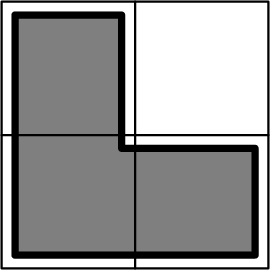
\includegraphics[width = 27.0mm]{img/fig0.png}
\end{center}
For which $n$ is it possible that, after some non-zero number of moves, the board has no stones?